\section{Alya and the combustion use case}
Alya is an HPC application for computational mechanics. It has diverse modules that solve a specific problem, which can be coupled to solve a general problem. For example, we can couple together the module to simulate how the temperature evolves in a system and the module that computes the particle motion in the same run. 

The code is written in Fortran90 and can use MPI, OpenMP/OmpSs and GPU. The module we are asked to optimize is pure MPI and despite the code is written in Fortran, it uses Cantera library for a critical computation inside the module. Cantera\cite{cantera} is an open-source suite of tools for problems involving chemical kinetics, thermodynamics, and transport processes written in C++.

The use case we will study consists of a bunsen flame in 2D. It is a simple use case although representative of the industrial real use cases of the application. Figure \ref{bunsen} a real picture of a bunsen flame. 

\begin{figure}[h]
  \centering
  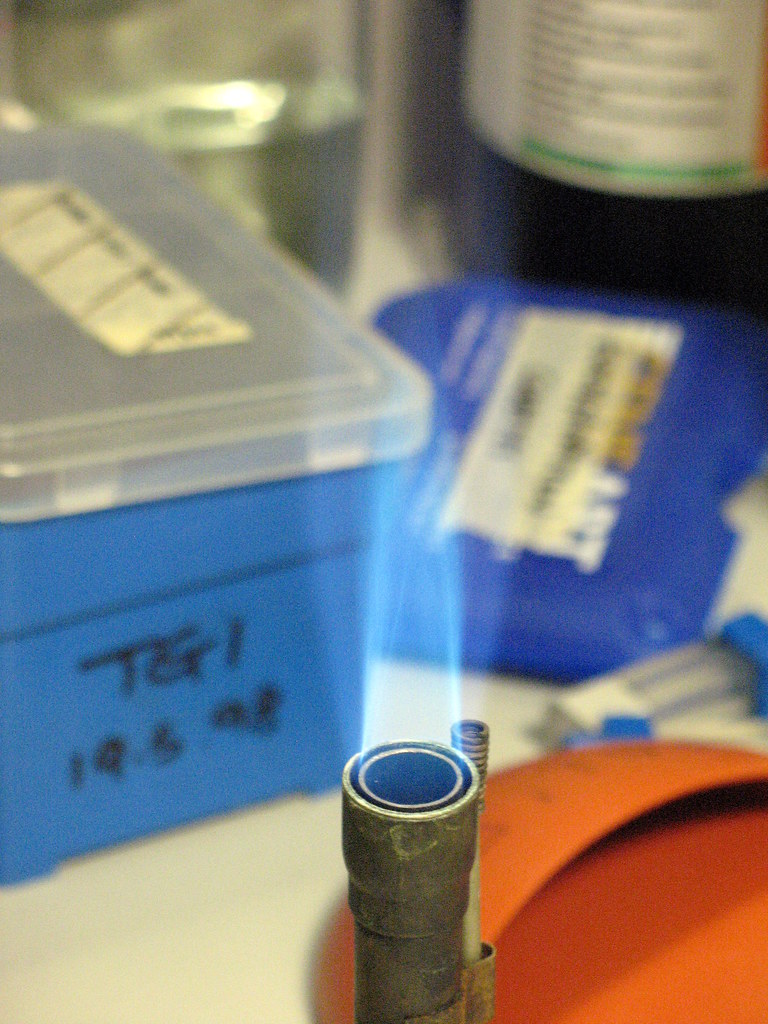
\includegraphics[width=0.5\textwidth]{bunsen}
  \caption[Bunsen flame]{Bunsen flame by El Bingle licensed under CC BY-NC-SA 2.0}
  \label{bunsen}
\end{figure}
  

In general terms the simulation consists of:
\begin{itemize}
  \item The centre of the 2D domain contains the bunsen flame.
  \item We compute environmental parameters such as temperature and pressure produced during the combustion for all the grid points.
  \item Following transport equations defined, compute the motion of chemical species, and if the environmental conditions are ideal, compute the chemical reactions.
\end{itemize}

Developers of the application gave us two versions of the bunsen 2D flame:

\begin{itemize}
  \item \textbf{Detailed:} It has a significant number of transport equations, which means that the case is industry-relevant and the chemical part of the simulation, will be the most relevant part of the code.

  \item \textbf{Reduced:} Has a short number of transport equations, meaning the computational relevance of the chemical part of the code is low, and the case is less industry-relevant but interesting to compare to the Detailed version.
\end{itemize}

